\documentclass[aspectratio=169,compress]{beamer}

\usepackage[utf8]{inputenc}
\usepackage{listings}
\usepackage{minted}
\usepackage{microtype}
\usepackage{amssymb}
\usepackage{tikz}
\usepackage{textcomp}
\usepackage[makeroom]{cancel}
\usepackage[most]{tcolorbox}
\usepackage{emoji}
\usepackage{booktabs}

\usepackage{bussproofs}
\EnableBpAbbreviations
\def\ScoreOverhang{1.5pt}
\def\proofSkipAmount{\vskip 0pt}
\def\defaultHypSeparation{\hskip0.75em}

% == Bibtex Setup ==
\usepackage[backend=biber,style=authoryear,maxcitenames=1,sorting=none]{biblatex}
\addbibresource{bib.bib}

% == Minted Setup ==
\usemintedstyle{trac}

% == Beamer Setup ==
\usecolortheme{rose}
\usefonttheme{metropolis} 
\beamertemplatenavigationsymbolsempty
\setbeamertemplate{footline}[frame number]
\setbeamercovered{transparent}
\usebackgroundtemplate{}

% == Commands Setup ==
\newcommand\Refl{\textsc{Refl}}
\newcommand\Taut{\textsc{Taut}}
\newcommand\Tautof[1]{\Taut\smash{\ensuremath{_{#1}}}}
\newcommand\TautT{\Tautof{\T}}
\newcommand\Trans{\textsc{Trans}}
\newcommand\Cong{\textsc{Cong}}
\newcommand\Bind{\textsc{Bind}}
\newcommand\Sko{\textsc{Sko}}
\newcommand\SkoEx{\Sko\smash{\ensuremath{_{\,\exists}}}}
\newcommand\SkoAll{\Sko\smash{\ensuremath{_{\,\forall}}}}
\newcommand\Let{\textsc{Let}}
\newcommand\OnePoint{\textsc{1Pt}}
\newcommand\OnePointEx{\OnePoint\smash{\ensuremath{_{\,\exists}}}}
\newcommand\OnePointAll{\OnePoint\smash{\ensuremath{_{\,\forall}}}}

\newcommand\vvthinspace{\kern+0.041667em}
\newcommand\vthinspace{\kern+0.083333em}
\newcommand\negvthinspace{\kern-0.083333em}
\newcommand\negvvthinspace{\kern-0.041667em}

\newcommand\All[2]{\forall #1.\;#2}
\newcommand\Ex[2]{\exists #1.\;#2}
\newcommand\Choicename{\varepsilon}
\newcommand\Choice[2]{\Choicename #1.\>#2}
\newcommand\judgei[1]{{\vartriangleright}\;#1}
\newcommand\judge[2]{#1\;\vthinspace{\vartriangleright}\;#2}
\newcommand\judgealti[1]{{\blacktriangleright}\;#1}
\newcommand\judgealt[2]{#1\;\vthinspace{\blacktriangleright}\;#2}
\newcommand\Not{{\lnot}\,}
\newcommand\limp{\rightarrow}

\newcommand\axiomstrut{\vrule height 1.25ex depth 0pt width 0pt} %% TYPESETTING

% Common Abbreviations
\newcommand\smtlib{SMT-LIB}

\title{Alethe: Towards a Generic SMT Proof Format}
\subtitle{PxTP 2021}
\author{
\textbf{Hans-Jörg Schurr}\inst{1},
Mathias Fleury\inst{2},
Haniel Barbosa\inst{3},
Pascal Fontaine\inst{4}
}

\institute{
    \inst{1}University of Lorraine, CNRS, Inria, and LORIA\and
    \inst{2}Johannes Kepler University Linz, Austria\and
    \inst{3}Universidade Federal de Minas Gerais, Belo Horizonte, Brazil\and
    \inst{4}Universit\'{e} de Liège
}

\tcbset{on line,
    boxsep=0pt, left=0pt,right=0pt,top=0pt,bottom=0pt,
    colframe=white,colback=orange!30,
    highlight math style={enhanced}
}

\date{July 11, 2021}

\begin{document}

\frame{\titlepage}

\note[itemize]{
    \item Say this is an effort that emerged over the last few month
    \item Mention other people are also involved
    \item Clarify for SMT!
}

\begin{frame}{Some History}
\begin{columns}
    \begin{column}{0.5\textwidth}
        \begin{block}{Within \raisebox{-0.21\height}{\includegraphics[scale=.12]{veritlogo}}}
            \begin{itemize}
                \item First: Ad-hoc (\emoji{scroll} TACAS 2006)
                \item Later: Redesigned (\emoji{scroll} PxTP 2011)
                \item Syntax changed over time
            \end{itemize}
        \end{block}
        \pause
        \begin{block}{SMTCoq}
            \begin{itemize}
                \item One of the first users
                \item Verified checker (\emoji{scroll} CPP 2011)
                \item Base for automation in Coq\\ (\emoji{scroll} CAV 2017, PxTP -3h20)
            \end{itemize}
        \end{block}
    \end{column}
    \begin{column}{0.5\textwidth}
        \pause
        \begin{block}{Fine-Grained Proofs and Isabelle}
          \begin{itemize}
            \item Support for reasoning with bound variables (\emoji{scroll} CADE 2017, JAR 2020)
            \item Typical for pre-processing in SMT
            \item Isabelle/HOL integration\\ (\emoji{scroll} CADE +49h40)
          \end{itemize}
        \end{block}
        \pause
        \begin{block}{Now!}
            \begin{itemize}
                \item[\emoji{skull}] Proofonomicon
                \item[\emoji{angel}] Speculative Specification
                \item[\emoji{feather}] It's now Alethe! (\emoji{scroll} PxTP -0h05)
            \end{itemize}
        \end{block}

    \end{column}
    
\end{columns}
\end{frame}

\note[itemize]{
    \item Say that it's not very scientific and that I probably miss some things
    \item Mention other people are also involved:
    \begin{itemize}
        \item Frédéric Besson and Laurent Théry, 
        \item David Déharbe and Bruno Woltzenlogel Paleo 
    \end{itemize}
    \item Clarify for SMT!
}

\begin{frame}[label=bird,plain]
    \begin{center}
        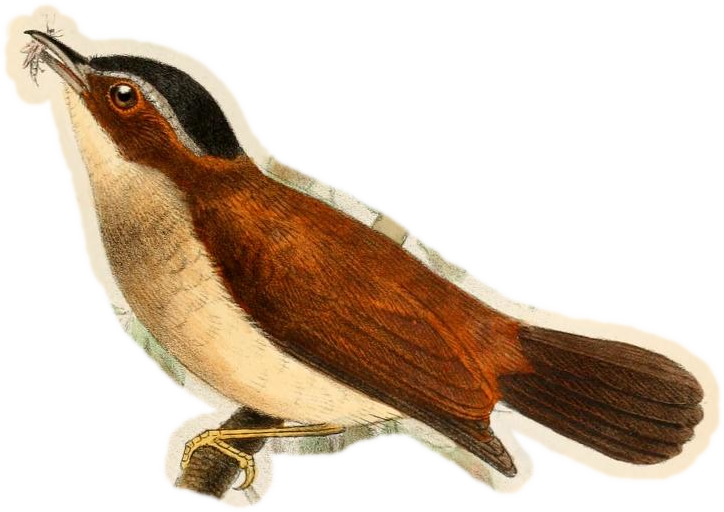
\includegraphics[scale=1.6]{alethe}
    \end{center}
\end{frame}

\begin{frame}[plain]
    \begin{center}
        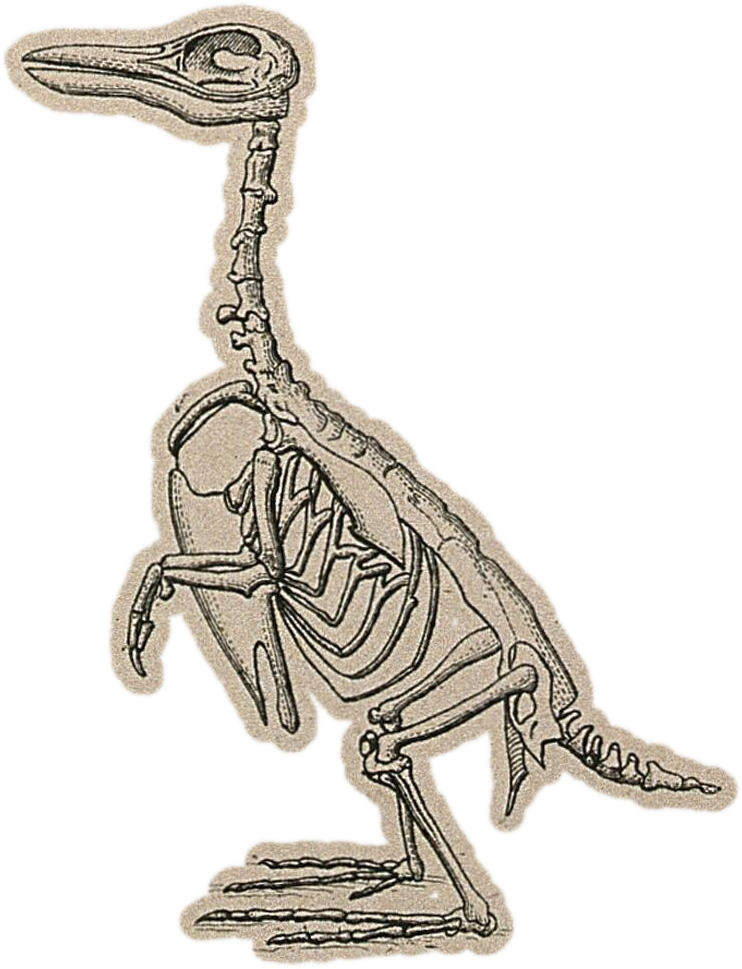
\includegraphics[scale=0.25]{skeleton}
    \end{center}
\end{frame}

\begin{frame}[fragile]{Basic Structur}
    \begin{columns}
        \begin{column}{0.4\textwidth}
{\Large
\[
    \AXC{$t_1$}
    \AXC{$t_2$}
    \UIC{$t_3$}
    \noLine
    \UIC{$\vdots$}
    \noLine
    \UIC{$\neg t_1$}
    \RightLabel{\normalsize\texttt{resolution}}
    \BIC{
        $\bot$
    }
    \DP
\]
}
        \end{column}
        \begin{column}{0.6\textwidth}
            \begin{center}
\begin{minted}[fontsize=\footnotesize]{smtlib2.py -x}
(assume a0 t1)
(assume a1 t2)
(step s1  (cl t3)
        :premises (a1)     :rule rule1)
   ...
(step s20 (cl (not t1))
        :premises (s19)    :rule rule2)
(step s21 (cl )
        :premises (a0 s20) :rule resolution)

\end{minted}

            \end{center}
        \end{column}
    \end{columns}
\end{frame}

\begin{frame}[fragile]{Subproofs With Assumptions}
    \begin{columns}
        \begin{column}{0.4\textwidth}
{\Large
\[
    \AXC{$t_1$}
    \UIC{$t_2$}
    \AXC{$[t_2]$}
    \noLine
    \UIC{$\vdots$}
    \noLine
    \UIC{$t_3$}
    \RightLabel{\normalsize\texttt{subproof}}
    \UIC{$\neg t_2, t_3$}
    \RightLabel{\normalsize\texttt{resolution}}
    \BIC{
        $t_3$
    }
    \DP
\]
}
        \end{column}
        \begin{column}{0.6\textwidth}
            \begin{center}
\begin{minted}[fontsize=\footnotesize]{smtlib2.py -x}
(assume a0 t1)
(step s1 (cl t2)
        :premises (a0)    :rule rule1)
(anchor :step s2)
  (assume s2.a1      t2)
   ...
  (step   s2.s10 (cl t3)
        :premises (s2.s9) :rule rule2)
(step s2 (cl (not t2) t3) :rule subproof)
(step s3 (cl t3)
        :premises (s1 s2) :rule resolution)
\end{minted}
            \end{center}
        \end{column}
    \end{columns}
\end{frame}

\begin{frame}[fragile]{Reasoning With Binders}
    \begin{columns}
        \begin{column}{0.4\textwidth}
%\newcommand\judge[2]{#1\;\vthinspace{\vartriangleright}\;#2}
{\Large
\[
    \AX$\fCenter$
    \RightLabel{\normalsize\texttt{refl}}
    \UI$x\mapsto y\;\vthinspace{\vartriangleright}\;\fCenter x=y$
    \RightLabel{\normalsize\texttt{cong}}
    \UI$x\mapsto y\;\vthinspace{\vartriangleright}\;\fCenter f(x)=f(y)$
    \RightLabel{\normalsize\texttt{bind}}
    \UI$\All{x}{f(x)}\fCenter\;=\All{y}{f(y)}$
    \DP
\]
}
        \end{column}
        \begin{column}{0.6\textwidth}
            \begin{center}
\begin{minted}[fontsize=\footnotesize]{smtlib2.py -x}
(anchor :step s2 :args ((:= (x S) y)))
  (step s2.s1 (cl (= x y))    :rule refl)
  (step s2.s2 (cl (= (f x) (f y)))
                              :rule cong)
(step s2 (cl (= (forall ((x S)) (f x))
                (forall ((y S)) (f y)))
                              :rule bind)
\end{minted}
            \end{center}
        \end{column}
    \end{columns}
\end{frame}

\againframe{bird}

\begin{frame}{Rules}
    \begin{block}{Current State}
    \begin{itemize}
        \item Overall 90 rules, mostly simple tautologies
        \item Seven categories -- with overlaps
        \item Some historic overhead
        \item[\emoji{building-construction}] Cleanup and normalization
    \end{itemize}
    \end{block}
    \pause
    \begin{block}{How can we accommodate different solvers?}
        \begin{itemize}
            \item Some solvers might be able to use rules more strictly.
            \item Example:
            \begin{itemize}
                \item $a = b \land b = c\limp a = c$
                \item $c = b \land a = b\limp a = c$
            \end{itemize}
            \item[\emoji{light-bulb}] Have an optional annotation to mark restricted usage.
        \end{itemize}
    \end{block}
\end{frame}

\begin{frame}{Tools}
    \begin{block}{A Checker and Elaborator}
    \begin{itemize}
        \item ``A second pair of eyes".
        \item Small, independent codebase -- in Rust.
        \item Long term: rewrite steps to their stricter form, framework
              to replace non-standard rules by standard rules.
        \item[\emoji{man}] Bruno Andreotti
    \end{itemize}
    \end{block}
    \pause
    \begin{block}{Support in \emph{cvc5}}
        \begin{itemize}
            \item Part of a wider effort to overhaul the proof module of \emph{cvc5}.
            \item Will add more theories to Alethe.
            \item[\emoji{woman}] Hanna Lachnitt and the wider \emph{cvc5} team.
        \end{itemize}
    \end{block}
\end{frame}

\begin{frame}[plain]
    \begin{columns}
        \begin{column}{0.28\textwidth}
        \end{column}
        \begin{column}{0.64\textwidth}
            \begin{block}{Speculative Specification}
                \texttt{http://www.verit-solver.org/alethe.pdf}
            \end{block}
            \begin{block}{Feedback}
                \texttt{https://gitlab.uliege.be/verit/alethe}
            \end{block}
        \end{column}
        \begin{column}{0.28\textwidth}
        \end{column}
    \end{columns}
\end{frame}

\end{document}
